%%%%%%%%%%%%%%%%%%%%%%%%%%%%%%%%%%%%%%%%%%%%%%%%%%%%%%%%%%%%%%%%%%%%%%%%%%%%%%%%%%%%%%%%%%%%%%%%%%%%%%%%%%%%%%%%%
\documentclass[12pt]{article}
\usepackage{latexsym,epsfig,graphicx,epstopdf,amsmath,amssymb,amscd,pifont, multirow,chicago,psfrag,paralist,dsfont,url}
\usepackage[titletoc]{appendix}
\usepackage{listings}

\usepackage{subcaption}
%\usepackage[labelformat=parens,labelsep=quad,skip=3pt]{caption}
\usepackage{graphicx}
\usepackage{bm}

\usepackage{varwidth}
\usepackage{verbatim}

\newenvironment{centerverbatim}{%
  \par
  \centering
  \varwidth{\linewidth}%
  \verbatim
}{%
  \endverbatim
  \endvarwidth
  \par
}


%%%%%%%%%%%%%%%%%%%%%%%%%%%%%%%%%%%%%%%%%%%%%%%%%%%%%%%%%%%%%%%%%%%%%%%%%%%%%%%%%%%%%%%%%%%%%%%%%%%%%%%%%%%%%%%%%
\textwidth  6.6in \textheight 9.2in \topmargin -0.6in \oddsidemargin
-0.0in \evensidemargin -0.0in \pagestyle{plain}

\newcommand{\cmark}{\ding{51}}%
\newcommand{\xmark}{\ding{55}}%
\newcommand{\thetavec}{{\boldsymbol{\theta}}}
\newcommand{\veps}{\varepsilon}
\newcommand{\loglik}{\mathcal{L}}
\newcommand{\vepsvec}{{\boldsymbol{\varepsilon}}}
\newcommand{\Sigmavec}{{\boldsymbol{\Sigma}}}
\newcommand{\wvec}{{\boldsymbol{w}}}
\newcommand{\zerovec}{{\boldsymbol{0}}}
\newcommand{\onevec}{{\boldsymbol{1}}}
\newcommand{\Ivec}{{\boldsymbol{I}}}
\newcommand{\betavec}{{\boldsymbol{\beta}}}
\newcommand{\betahat}{{\widehat{\beta}}}
\newcommand{\etavec}{{\boldsymbol{\eta}}}
\newcommand{\thetavecC}{{\boldsymbol{\theta}_C}}
\newcommand{\thetavecT}{{\boldsymbol{\theta}_T}}
\newcommand{\thetaveca}{\thetavec_{1}}
\newcommand{\thetavecb}{\thetavec_{2}}
\newcommand{\EE}{\mathbb{E}}
\newcommand{\Bset}{\mathbf{B}}
\newcommand{\Xset}{\mathbf{X}}
\newcommand{\Xmat}{\mathbf{X}}
\newcommand{\Cmat}{\mathbf{C}}
\newcommand{\Zmat}{\mathbf{Z}}
\newcommand{\Pmat}{\mathbf{P}}
\newcommand{\Hmat}{\mathbf{H}}
\newcommand{\pvec}{\boldsymbol{p}}
\newcommand{\Sset}{\mathbf{S}}
\newcommand{\cp}{{\textrm{CP}}}
\newcommand{\pr}{{\textrm{Pr}}}
\newcommand{\mvn}{{\textrm{MVN}}}
\newcommand{\mse}{{\textrm{MSE}}}
\newcommand{\emse}{{\textrm{EMSE}}}
\newcommand{\TAE}{{\textrm{TAE}}}
\newcommand{\MAE}{{\textrm{MAE}}}
\newcommand{\bin}{{\textrm{bin}}}
\newcommand{\enum}{{\textrm{enum}}}
\newcommand{\Var}{{\textrm{Var}}}
\newcommand{\muhat}{\widehat{\mu}}
\newcommand{\sigmahat}{\widehat{\sigma}}
\newcommand{\thetavechat}{\widehat{\thetavec}}
\newcommand{\thetavecmis}{\thetavec_{\ast}}
\newcommand{\mumis}{\mu_{\ast}}
\newcommand{\sigmamis}{\sigma_{\ast}}
\newcommand{\thetavecahat}{\widehat{\thetavec}_1}
\newcommand{\thetavecbhat}{\widehat{\thetavec}_2}
\newcommand{\amse}{{\textrm{AMSE}}}
\newcommand{\avar}{{\textrm{AVar}}}
\newcommand{\abias}{{\textrm{ABias}}}
\newcommand{\bias}{{\textrm{Bias}}}
%\newcommand{\diag}{{\textrm Diag}}
\newcommand{\Arg}{{\textrm{Arg}}}
\newcommand{\Ber}{{\textrm{Ber}}}
\newcommand{\atantwo}{{\textrm{atan2}}}
\newcommand{\ivec}{{\boldsymbol{i}}}
\newcommand{\dgoto}{\overset{d}{\rightarrow}}
\newcommand{\Pgoto}{\overset{P}{\rightarrow}}
\newcommand{\asgoto}{\overset{a.s.}{\longrightarrow}}
\newcommand{\sev}{\textrm{sev}}
\newcommand{\nor}{\textrm{nor}}
\newcommand{\N}{\textrm{N}}
\newcommand{\diag}{\textrm{Diag}}
\newcommand{\PMD}{\textrm{PMD}}
\newcommand{\wh}{\widehat}
\newcommand{\sigmaR}{\sigma_{R}}
\newcommand{\muR}{\mu_{R}}
\newtheorem{result}{Result}
\newcommand{\Xvec}{\boldsymbol{X}}
\newcommand{\Zvec}{\boldsymbol{Z}}
\newcommand{\xvec}{\boldsymbol{x}}
\newcommand{\kvec}{\boldsymbol{k}}
\newcommand{\rvec}{\boldsymbol{r}}
\newcommand{\hvec}{\boldsymbol{h}}
\newcommand{\muvec}{\boldsymbol{\mu}}
\newcommand{\minitab}[2][l]{\begin{tabular}{#1}#2\end{tabular}}
\newcommand{\fft}{\textrm{FFT}}
\newcommand{\code}{\texttt}


%mu sigma vector
\newcommand{\Sig}{\boldsymbol{\Sigma}}
\newcommand{\mvec}{\boldsymbol{\mu}}

%methods
\newcommand{\SIM}{{\textrm{SIM}}}
\newcommand{\NA}{{\textrm{NA}}}
\newcommand{\dft}{{\textrm{DFT-CF}}}



\newcommand{\qed}{\hfill\blacksquare}
\newcommand{\qedw}{\hfill \ensuremath{\Box}}


%%%%%%%%%%%%%%%%%%%%%%%%%%%%%%%%%%%%%%%%%%%%%%%%%%%%%%%%%%%%%%%%%%%%%%%%%%%%%%%%%%%%%%%%%%%%%%%%%%%%%%%%%%%%%%%%%
\def\baselinestretch{1.25}
\renewcommand{\arraystretch}{.8}
%%%%%%%%%%%%%%%%%%%%%%%%%%%%%%%%%%%%%%%%%%%%%%%%%%%%%%%%%%%%%%%%%%%%%%%%%%%%%%%%%%%%%%%%%%%%%%%%%%%%%%%%%%%%%%%%%

\usepackage[ruled,vlined]{algorithm2e}
%%%%%%%%%%%%%%%%%%%%%%%%%%%%%%%%%%%%%%%%%%%%%%%%%%%%%%%%%%%%%%%%%%%%%%%%%%%%%%%%%%%%%%%%%%%%%%%%%%%%%%%%%%%%%%%%%

%\theoremstyle{definition}
%\newtheorem{exmp}{Example}[section]



\newtheorem{example}{Example}
\newtheorem{thm}{Theorem}
\newtheorem{ppt}{Proposition}
\newtheorem{lemma}{Lemma}
\newtheorem{remark}{Remark}
\newtheorem{defn}{Definition}
\newtheorem{corl}{Corollary}

%%%%%%%%%%%%%%%%%%%%%%%%%%%%%%%%%%%%%%%%%%%%%%%%%%%%%%%%%%%%%%%%%%%%%%%%%%%%%%%%%%%%%%%%%%%%%%%%%%%%%%%%%%%%%%%%%
\def\baselinestretch{1.25}
\renewcommand{\arraystretch}{.8}
%%%%%%%%%%%%%%%%%%%%%%%%%%%%%%%%%%%%%%%%%%%%%%%%%%%%%%%%%%%%%%%%%%%%%%%%%%%%%%%%%%%%%%%%%%%%%%%%%%%%%%%%%%%%%%%%%

\setcounter{tocdepth}{2}

%-------------------------------------------------------------------------
\begin{document}
%%%%%%%%%%%%TITLE%%%%%%%%%%%%%%%%%%%%%%%%%%%%%%%%%%%

%\title{The Computing of Probability Mass Functions for the Poisson Multinomial Distribution}

\title{The Poisson Multinomial Distribution and Its Applications in Voting Theory, Ecological Inference, and Machine Learning}


%\iffalse
\author{
Zhengzhi Lin, Yueyao Wang, and Yili Hong\\[1.5ex]
{Department of Statistics, Virginia Tech, Blacksburg, VA 24061}
}
%\fi
	
\date{\today}
	
\maketitle
	%%%%%%%%%%%%%%%%%%%%%%%%%%%%%%%%%%%%%%%%%%%%%%%%%%%%%%%%%%%%%%%%%%%%%%%%%%%%%%%%%%%%%%%%%%%%%%%%%%%%%%%%%%%%%%%%
\begin{abstract}
The Poisson multinomial distribution (PMD) can be considered as a sum of independent categorical distributions that have same categories. The $\PMD$ is useful in many areas such as, voting theory, ecological inference and machine learning. The distribution functions of $\PMD$, however, is usually difficult to compute. In this paper, we develop methods to compute the probability mass function (pmf) for PMD using Fourier transformation, normal approximation and simulation. We study the accuracy and efficiency of the methods and give recommendations for the methods to be used under corresponding circumstances. We also illustrate three applications of PMD in voting theory, aggregated data inference and soft classification. We build an R package to implement our methods and illustrate the package with examples.

\textbf{Key Words:} Poisson Binomial Distribution; Machine Learning; Classification; Uncertainty Quantification; Ecological Inference;  Aggregated Data Inference; Political Science;  Voting Theory
\end{abstract}
	
	%%%%%%%%%%%%%%%%%%%%%%%%%%%%%%%%%%%%%%%%%%%%%%%%%%%%%%%%%%%%%%%%%%%%%%%%%%%%%%%%%%%%%%%%%%%%%%%%%%%%%%%%%%%%%%%%%%%%%
%\newpage
%\tableofcontents
\newpage
	
	%%%%%%%%%%%%%%%%%%%%%%%%%%%%%%%%%%%%%%%%%%%%%%%%%%%%%%%%%%%%%%%%%%%%%%%%%%%%%%%%%%%%%%%%%%%%%%%%%%%%%%%%%%%%%%%%%%%%%
\section{Introduction}
\subsection{Motivation}

Suppose there are $n$ random variables follow independent but not identical categorical distributions that have the same sample space. Then the sum of the random variables follows $\PMD$. For example, there are $n$ independent balls, and one needs to throw them into $m$ different bins. Each ball has its own probabilities of falling into a specific bin. Then the probability distribution of the ball counts in each bin is $\PMD$. $\PMD$ is a generalization of multinomial distribution. In addition, when $m=2$ the $\PMD$ reduces to the Poisson binomial distribution.

$\PMD$ has applications in many fields including computer science, probability, statistics and political science. It has applications in game theory (\citeNP{Cheng2017PlayingAG}), digital imaging (\citeNP{akter2019double}), machine learning (\citeNP{kamath2014learning}), etc. One of the intriguing areas that involves $\PMD$ is political science. It would be good to illustrate $\PMD$ further via a very simple example in election scenario. 

Suppose a committee with $n$  independent members needs to elect a chairman between $m$ candidates. Each member has different voting behavior. Mostly, people pay attention to the result of an election while statisticians focus on the probability for each electoral outcome to happen. $\PMD$ is a perfect model for this example by seeing members as independent random variables following different categorical distributions which have the same categories. Explicitly,  each member has its own probability to vote for a specific candidate. A electoral result here is the number of votes each candidate gets at the end of the election. In such an election, what will be the most likely electoral result? What possibility does a specific candidate have to win the election? These question are usually of the greatest concern and often hard to answer. In total, there will be $\binom{n+m-1}{m-1}$ different electoral results. The probability mass function (pmf) of $\PMD$ is composed of probabilities of all different electoral results. Therefore, if we are able to compute the pmf of $\PMD$, the questions will be easily solved.

Additionally, in machine learning, people often encounter the needs of classifying data into different categories. Suppose a model computes probabilities of an observation falling into $m$ categories, the decision is usually made by selecting the category that has the highest probability. In uncertainty quantification context, people introduce randomness in the decision making process.  The decision will be the random sample drew from a $m$-dimension categorical distribution with respect to computed probabilities. If we have $n$ data points, there will be $n$ independent categorical distributions. In this case, people consider the counts of points the classifier put into each category and form a confusion matrix. $\PMD$ is a perfect tool to characterize the probability distribution of the counts in the confusion matrix.

In ecological inference, consider making statistical inference to aggregated data. An aggregated dataset is to separate data points into groups and consider the groups as new data points. Let's assume the data response variable is categorical. In the grouped dataset, we can count the number of each category in each group and take it as our new response variable and this variable will follow $\PMD$ accordingly. All the areas above that involve $\PMD$ also require computation of its probability mass function. Without the pmf, we are unable to draw any conclusion over the discussed examples.

Enumeration can be a way because if $n \times m$ is small we can list all outcomes by hand. However, when $n$ and $m$ increase, the computing will be a dilemma that is impossible to overcome by enumeration. Thus arises the need of methods that are computationally cheap and precise at the meantime. Not only in the fields mentioned above, computing pmf is frequently required in many scenarios that $\PMD$ are involved. There is no existing algorithm for computing pmf for PMD. Hereby we are motivated to build one that can calculate pmf of $\PMD$ efficiently.



\subsection{Related Literature and Contribution of This Work}

%Ecological inference https://www.pnas.org/content/96/19/10578

Some former studies have uncovered $\PMD$'s structure and some of its properties. In 2015, \citeN{Daskalakis2015OnTS} proved that $\PMD$ is $\epsilon$-cover, which means there exists a set of distributions small enough to cover the set of all $\PMD$s. $\PMD$ can also be $\epsilon$-close so that it can be approximated by other distributions. The paper also reveal that exists learning algorithms for $\PMD$s. This result shows that we can find a sampling scheme to draw enough samples out of a $\PMD$ to depict its structure and complexity. Simply saying, we could study $\PMD$'s probability mass function via sampling. At almost the same time, \citeN{diakonikolas2016fourier} obtained a different understanding of the structures of $\PMD$s' using Fourier transformation and disclosed the sparsity of $\PMD$. The paper also provided the first computationally efficient for $\PMD$s and showed central limit theorem (CLT) can be applied to $\PMD$. The most important statistical characteristic of $\PMD$, probability mass function has not been explored yet. \citeN{Hong2013} consider the exact and approximate methods for computing the pmf of the Poisson binomial distribution. \citeN{zhang2018generalized} introduce the general Poisson binomial distribution and develop an algorithm to compute its distribution functions.

Current studies have shown that $\PMD$s can be applied to many fields. In game theory, based on the structure and properties of $\PMD$, \citeN{diakonikolas2016fourier} constructed a efficient scheme to approximate Nash equilibria in anonymous games and \citeN{Cheng2017PlayingAG} proved that any $n$-player anonymous games can have approximate Nash equilibria in polynomial time. \citeN{akter2019double} introduced $\PMD$ in image processing field for the first time. They used $\PMD$ to count the encrypted image data and computed $\PMD$'s probability mass functions to obtain optimal results. However, the probability mass function of $\PMD$ is computed by using simplified multinomial distributions which is actually an approximation method.

In this paper, the contributions are following. The main contribution of this paper is constructing an exact method that uses fast Fourier transformation algorithm (FFT) to compute pmf of $\PMD$.  We call this method $\dft$. Besides, we also construct two approximation methods to compute pmf of $\PMD$, the one is a simulation scheme and the other one is approximation based on CLT. Along the journey of constructing methods, several properties and theorems are built.

Specifically, the $\dft$ method applies multidimensional discrete Fourier transformation to the characteristic function (cf) of $\PMD$ to obtain its pmf. The method $\NA$ uses CLT to approximate pmf of $\PMD$. We prove an analytic error bound for this method based on its CLT converge rate. The $\SIM$ method is the other approximation method. $\SIM$ uses multiple multinomial distributions to simulate $\PMD$ and obtains pmf via simulation results. An expected absolute error bound of this method is provided and proved.

We also studying accuracy and time efficiency of each methods under different scenarios. Since there is no way to compute true pmf for $\PMD$, the logic of accuracy study is as following. We explore the situations under which we are able to compute the pmf of $\PMD$ and construct accuracy test for $\dft$. Then we use $\dft$ as our true pmf to conduct accuracy tests for other methods. For time efficiency, we only test the $\dft$ method since it is the only method that automatically compute the whole pmf while others only compute partial pmf (eg. a single probability mass point). We give $m=2,3,4,5$ and let $n$ grow sufficiently large while we record the time $\dft$ takes to finish computing.

Accuracy test for $\dft$ is conducted by using binomial, Poisson binomial and small dimensional $\PMD$s. It suffices to show $\dft$ is pretty accurate and the error comes from the fast Fourier transformation algorithm. Due to computational limitation, accuracy test for $\SIM$ is done by setting $m=3$ and $n$ to be moderately large. Result shows that the method is accurate and the error bound can be controlled via improving simulation repeating times. Through setting $m=3,5,7$ and letting $n$ be sufficiently large, our accuracy test support $\NA$'s accuracy when $n$ is moderate and large.

Then we separate all $\PMD$s into different subsets according to their dimensions and give out recommendations with respect to which method to be chosen. Based on our developed methods, we make applications in the fields of ecological inference, political science and classification.

In ecological inference, people separate the data into multiple groups and consider each group as a new data point, this is also called aggregated data. We use the Predictive Maintenance Dataset Data Set \cite{Dua:2019} from UCI machine learning repository to conduct the application of $\PMD$ in ecological inference, the dataset is separated into several groups to form aggregated data and a logistic type model is build.

We also provide an example of applying $\PMD$ in voting scenario. The probability of a voting result can be computed via $\PMD$. Thus $\PMD$ provide a new perspective of predicting electoral results.

We illustrate an application of $\PMD$ in soft classification context using Electroluminescence (EL) image data. We show that $\PMD$ is a good tool to describe the distribution of the counts in confusion matrix.

We build an R package to contain all methods we develop and demonstrate the usage of the package.






\subsection{Overview}
The rest of the paper is organized as follows. In section \ref{sec:pmd}, we describe the mathematical definition of Poisson Multinomial distribution and list some of its statistical properties. In section \ref{sec:CA.driving.study}, we demonstrate the details of  the three methods that we develop to compute $\PMD$'s pmf.  The section \ref{sec:Method Comparisons} studies the curacy and time efficiency characteristics of the three methods, we also give out recommendations of preferred situations for each method. In the section \ref{sec:applications}, we illustrate application of our methods via three examples respectively in the fields of voting theory, ecological inference and soft classification. In the section \ref{sec:rpackage}, we introduce our R package that implemented with the methods and the section \ref{sec:conclusion} concludes the paper and lists prospective research areas.




%%%%%%%%%%%%%%%%%%%%%%%%%%%%%%%%%%%%%%%%%%%%%%%
\section{Poisson Multinomial Distribution} \label{sec:pmd}
%%%%%%%%%%%%%%%%%%%%%%%%%%%%%%%%%%%%%%%%%%%%%%%%%%%%%%%%%%%%%%%%%%%%%%%%%%%%%%%%%%
\subsection{Definition of the Distribution}
Suppose there are $n$ mutually independent multinomial experiments with the following properties. Each of the multinomial experiments only has one trial and the outcome will be one of $m$ categories. Let $\Ivec_{i} = (I_{i1}, \dots, I_{im})', i=1, \dots, n$ be random indicator vectors to denote the outcomes of the multinomial experiments described above. Also, let the associated probability vectors be $\pvec_{i} = (p_{i1}, \dots, p_{im})'$. Correspondingly, for a fixed $i$ we have $\sum_{j=1}^{m}p_{ij}=1$ and $\sum_{j=1}^{m}I_{ij}=1$.


 The we say the sum $\Xvec = (X_{1}, \dots, X_{m})'= \sum_{i=1}^{n}\Ivec_{i}$ follows a PMD. We denote the distribution as
$$\Xvec \sim \PMD(\Pmat).$$ where $X_{j} = \sum_{i=1}^{n} I_{ij}, j=1,\dots,m$. The matrix $\Pmat$ is called success probability matrix (SPM).

%\begin{equation*}
%\Pmat_{n \times m} = \begin{pmatrix}
%p_{11} &  \dots & p_{1m} \\
%\vdots & \ddots & \vdots \\
%p_{n1} &  \dots & p_{nm} \\
%\end{pmatrix}.
%\end{equation*}

\begin{equation*}
\Pmat = (\pvec_{1}, \dots, \pvec_{n} )'.
\end{equation*}

Note that the random variables, $X_1, \dots, X_{m}$ satisfy the following constraint $$\sum_{j=1}^{m}X_{j} = n.$$ Hence we can replace one of them, for example, $X_m$ with $n-\sum_{j=1}^{m-1}X_j$.

Let $\xvec = (x_1,\dots,x_m)'$ be a realization of a $\PMD$ random variable $\Xmat$. The probability mass function (pmf) of PMD is defined as,
$$\text{Pr}(\Xmat=\xvec) = \text{Pr} \left( X_1 = x_1, \dots, X_m = x_{m-1}, X_{m} = n-\sum_{i=1}^{m}x_i \right).$$

Here we give a simple example in election to illustrate the calculation of the pmf by hand.
\begin{example}%\normalfont
Suppose there are three candidates and four voters. The result of voting is a random variable $\Xmat \sim \PMD(\Pmat)$. Based on historical information, the SPM is obtained as 
\begin{equation*}
\Pmat_{4 \times 3} = \begin{pmatrix}
0.1 &  0.2 & 0.7\\
0.5 & 0.2 & 0.3\\
0.4 &  0.5 & 0.1\\
0.8 & 0.1 & 0.1
\end{pmatrix}.
\end{equation*}
There are 15 distinct outcomes of the election. That is, the pmf is composed of 15 distinct non-zero mass points. It is trivial to compute the pmf of $\Xmat$ through enumeration. For example, the probability of a result that the first candidate gets 4 votes and others gets 0 vote, that is, $\xvec =  (4,0,0)'$.
\begin{equation*}
P\left( \Xmat = \xvec \right) = 0.1\times 0.5 \times 0.4 \times 0.8 = 0.016.
\end{equation*}
Also, if we take $\xvec=(1,3,0)'$, the probability of $\Xmat = \xvec$ is
\begin{align*}
P\left( \Xmat = \xvec \right)  =  & 0.1\times 0.2 \times 0.5 \times 0.1 +
 0.5\times0.2\times0.5 \times 0.1 \\
 & + 0.4\times0.2\times0.2\times0.1 + 0.8\times0.2\times0.2\times0.5 = 0.0236.
\end{align*}
%\qedw
\end{example}

When the dimension of $\Pmat$ is small, enumeration is an exact way to calculate the probability mass function. However, as $n \times m$ gets larger enumeration becomes impossible since we will have to compute $\binom{n+m-1}{m-1}$ possible outcomes which is calculated by the number of non-negative integer solution for equation $x_1 + \dots + x_m = n$.

For some special cases, when the SPM is identical across all rows, that is, $I_{i}$, $i = 1, \dots n$ are identically distributed, the distribution of $X$ can be simplified as multinomial distribution. Hence, the $\PMD$ is a generalization of the multinomial distribution. When $m=2$, the $\PMD$ is reduced to the Poisson binomial distribution.

In related literature, \citeN{Hong2013} consider the exact and approximate methods for computing the pmf of the Poisson binomial distribution. \citeN{zhang2018generalized} introduce the general Poisson binomial distribution and develop an algorithm to compute its distribution functions.


\subsection{Properties of the Distribution}
Now let us study some basic properties of Poisson multinomial distribution. 

\begin{ppt}%\normalfont
Suppose $\Xmat \sim \PMD (\Pmat)$, the mean of $\Xmat$ is
   $$\EE(\Xmat) = \muvec = \left( p_{\cdot1} ,\dots,p_{\cdot,m-1},p_{\cdot m}\right)'$$ where $p_{\cdot k} = \sum_{i=1}^{n}p_{i k}$.\\
The variance-covariance matrix of $\Xmat$ denoted by $\Sig$ is an $m \times m$ matrix that has entries $\sigma_{ij}$ defined as
\begin{equation*}
   \sigma_{ij} =
           \begin{cases}
             \sum_{k=1}^{n}p_{ki}(1-p_{ki}) & \quad \text{if } i=j\\
             -\sum_{k=1}^{n}p_{ki}p_{kj} & \quad \text{if } i \neq j\\
           \end{cases}.
\end{equation*}\\
For $\xvec = (x_1, \dots, x_m)'$, denote the probability $\Pr \left(\Xmat = \xvec \right)$ as $p(x_1,\ldots,x_{m})$. The characteristic function (cf) for the $\PMD$ is
%\begin{equation*}
%\phi_{\xvec}(t_1, \dots, t_{m-1})  =  \sum_{x_1 = 0}^{n} \cdots \sum_{x_{m-1} = 0}^n p(x_1,\ldots,x_{m-1})\exp\left(\ivec\sum_{j=1}^{m-1}t_jx_j\right).
%\end{equation*}

\begin{equation*}
\phi_{\xvec}(t_1, \dots, t_{m})  =  \sum_{x_1 = 0}^{n} \cdots \sum_{x_{m} = 0}^n p(x_1,\ldots,x_{m})\exp\left(\ivec\sum_{j=1}^{m}t_jx_j\right).
\end{equation*}

where  $\ivec=\sqrt{-1}$.
%\qedw
\end{ppt}
The derivations of mean and characteristic function are as trivial as following the definitions. The $\Sig$ can be calculated by observing that for any fix $i=1,\dots,n$, $I_{ij}$ and $I_{ik}$ has covariance $-p_{ij}p_{ik},j=1,\dots,m,k=1,\dots,m$. One important thing is that the covariance matrix $\Sig$ is singular because the elements of $\Xvec$ are linear dependent.

Notice that $\sum_{j=1}^{m}X_j = n$, without loss of generality, let $\Xvec^{\ast}=(X_1,\dots,X_{m-1})'$ with corresponding $\xvec^{\ast} = (x_1,\dots,x_{m-1})'$ and $\Pmat^{\ast}$ equals to the first $m-1$ columns of $\Pmat$. That is to define
$$
\Pmat^{\ast} = \left(\pvec_1^{\ast},\dots, \pvec_n^{\ast} \right)'.
$$
where $\pvec_{i}^{\ast} = \left(p_{i1},\dots,p_{i,m-1} \right)', i = 1,\dots,n$.

Then we denote the non-singular $(m-1) \times (m-1)$ covariance matrix of $\Xvec^{\ast}$ as $\Sigmavec^{\ast}$. We have
 $$\Var(\Xvec^{\ast}) =\Sig^{\ast}=\sum_{i=1}^n[\diag(\pvec_i^{\ast})-\pvec_i^{\ast} \pvec_i^{\ast \prime} ].$$
where $\pvec_i^{\ast}$ is the $i$th row of $\Pmat^{\ast}$. Also, we denote the mean of $\Xvec^{\ast}$ as $\mu^{\ast}$, then
  $$\EE(\Xvec^{\ast}) =\muvec^{\ast} = \left( p_{\cdot1} ,\dots,p_{\cdot,m-1}\right)'.$$
 In addition, the cf of $\Xvec^{\ast}$ is 
 \begin{equation*}
\phi_{\xvec^{\ast}}(t_1, \dots, t_{m-1})  =  \sum_{x_1 = 0}^{n} \cdots \sum_{x_{m-1} = 0}^n p(x_1,\ldots,x_{m-1})\exp\left(\ivec\sum_{j=1}^{m-1}t_jx_j\right).
\end{equation*}
 
\begin{ppt}%\normalfont
If the SPM $\Pmat$ can be written as a combination of diagonal matrices $\Pmat_1, \Pmat_2, \dots, \Pmat_{S}$, $\Pmat = \diag(\Pmat_{k}), k=1,\dots,S$. Then the outcome of $\Pmat$, $\xvec$ can hereby be decomposed in to outcomes of the diagonal matrices, $\xvec= (\xvec_{1},\dots,\xvec_{S})$.  There will also have random variables $\Xvec_{i} \sim \PMD(\Pmat_{i})$, respectively. The pmf can computed as the product of the corresponding marginal pmfs. That is
\begin{align*}
\Pr(\Xvec=\xvec)= \Pr(\Xvec_{1}=\xvec_{1}, \dots, \Xvec_{S}=\xvec_{S})= \prod_{k=1}^S \Pr(\Xvec_{k} = \xvec_{k}).
\end{align*}
%\qedw
\end{ppt}

To show this, we assume $\Pmat$ is $n \times m$ and $\Pmat_{k}$ is $n_k \times m_k$. $\sum_{k=1}^S n_k = n$ and $\sum_{k=1}^S m_k = m$. Suppose there are $n$ voters to vote $m$ candidates, certain groups of voters only vote for certain groups of candidates and there are no overlaps . Heuristically, we can separate candidates and voters into independent groups, in each group $k$, $k = 1,\dots,S$, voters voting for corresponding candidates described by probability matrix $\Pmat_{k}$. Strict proof can be done by decomposition of characteristic function of $\Pmat$ into characteristic functions of $\Pmat_{k}$'s.



\section{Computation of The Probability Mass Function} \label{sec:CA.driving.study}
%%%%%%%%%%%%%%%%%%%%%%%%%%%%%%%%%%%%%%%%%%%%%%%%%%%%%%%%%%%%%%%%%%%%%%%%%%%%%%%%%%%%
We introduce three methods for computing the pmf, which are the method based on multidimensional discrete Fourier transform ($\dft$), the normal approximation ($\NA$) method, and simulation based method ($\SIM$). $\dft$ is an exact method while the other two are approximate methods.

%%%%%%%%%%%%%%%%%%%%%%%%%%%%%%%%%%%%%%%%%%%%%%%%%%%%%%%%%%%%%%%%%%%%%%%%%%%%%%%%%%%%%%%%%%%%%%%%%%
\subsection{The $\dft$ Method}
%%%%%%%%%%%%%%%%%%%%%%%%%%%%%%%%%%%%%%%%%%%%%%%%%%%%%%%%%%%%%%%%%%%%%%%%%%%%%%%%%%%%%%%%%%%%%%%%%%
Although $\PMD$ is of great importance, its pmf is obscure and no straightforward form has been found so far. However, its characteristic function (cf) can be wrote down in an accessible form. The cf is just a Fourier transformation of pmf, thus we can obtain pmf via Fourier transformed cf. Notice the pmf is discrete, so the discrete Fourier transformation will be used. In this section we provide an exact method to compute the pmf of the PMD using multidimensional discrete Fourier transformation. To speed up the computing, we implement fast Fourier transformation algorithm (\citeNP{1386650}).

Suppose a random variable $\Xvec =  (X_1, \dots, X_{m})' \sim \PMD(\Pmat)$, where $\Pmat = (p_{ij})$, $i=1,\dots,n,j=1,\dots,m$. Equivalently, consider $\Xvec^{\ast} = (X_1, \dots, X_{m-1})'$ will be equivalent since the last element of $\Xvec$ is redundant. The cf of $\Xvec^{\ast}$ is

\begin{align}
\phi(t_1, \dots, t_{m-1}) & = \EE\left[\exp\left(\ivec\sum_{j=1}^{m-1}t_jX_j\right)\right]=\EE\left[\exp\left(\ivec\sum_{i = 1}^n \sum_{j=1}^{m-1}t_j I_{ij}\right)\right].
\end{align}
Here $\ivec=\sqrt{-1}$. We notice
\begin{equation}
\begin{split}
  &\EE\left[\exp\left(\ivec\sum_{j=1}^{m-1}t_jX_j\right)\right] = \sum_{x_1 = 0}^{n}\cdots \sum_{x_{m-1} = 0}^n p(x_1,\ldots,x_{m-1})\exp\left(\ivec\sum_{j=1}^{m-1}t_jx_j\right).\\
\end{split}
\end{equation}
By definition,
\begin{equation}
\exp\left(\ivec\sum_{j=1}^{m-1}t_jX_j\right)= \exp\left(\ivec\sum_{i = 1}^n \sum_{j=1}^{m-1}t_j I_{ij}\right)
\end{equation}
The expectation of RHS of (3) can be expressed as
\begin{equation}
\begin{split}
  &\EE\left[\exp\left(\ivec\sum_{i = 1}^n \sum_{j=1}^{m-1}t_j I_{ij}\right)\right] = \EE\left[ \exp\left( \ivec\sum_{j=1}^{m-1} t_jI_{1j} + \dots + \ivec\sum_{j=1}^{m-1} t_jI_{nj}\right)\right].\\
  \\
  & = \prod_{i=1}^n \EE\left[ \exp\left( \ivec \sum_{j=1}^{m-1} t_j I_{ij}\right)\right] = \prod_{i=1}^n \left[(1 - \sum_{j=1}^{m-1}p_{ij})+\sum_{j=1}^{m-1}p_{ij}\exp(\ivec t_j)\right].
\end{split}
\end{equation}
We know (4) is equivalent to (2). Therefore we get

\begin{align*}
\sum_{x_1 = 0}^{n}\cdots \sum_{x_{m-1} = 0}^n p(x_1,\ldots,x_{m-1})\exp\left(\ivec\sum_{j=1}^{m-1}t_jx_j\right)= \prod_{i=1}^{n}\left[(1 - \sum_{j=1}^{m-1}p_{ij})+\sum_{j=1}^{m-1}p_{ij}\exp(\ivec t_j)\right].
\end{align*}
Let $t_j = \omega l_j$, $l_j = 0, \ldots, n$, $\omega = 2\pi/(n+1)$. Then the equation becomes
\begin{align}
\frac{1}{(n+1)^{m-1}} \sum_{x_1 = 0}^{n}\cdots \sum_{x_{m-1} = 0}^n p(x_1,\ldots,x_{m-1}) \exp\left(\ivec\omega\sum_{j=1}^{m-1}l_j x_j\right)= \frac{1}{(n+1)^{m-1}} q(l_1, \ldots, l_{m-1}),
\end{align}
where
$$ q(l_1, \ldots, l_{m-1})=\prod_{i=1}^{n}\left[(1 - \sum_{j=1}^{m-1}p_{ij})+\sum_{j=1}^{m-1}p_{ij}\exp(\ivec \omega l_j)\right].$$	
Note that $q(l_1, \ldots, l_{m-1})$ can be computed directly. The left side of equation (5) is the inverse multi-dimensional discrete Fourier transform of the sequence $ p(x_1,\ldots,x_{m-1}), x_i = 0 , \dots, n$. Therefore we can apply Multi Dimensional Discrete Fourier Transformation(MD-DFT) on both sides to recover the sequence, the pmf can be obtained as
\begin{equation}
p(x_1, \ldots, x_{m-1}) = \frac{1}{(n+1)^{m-1}}\sum_{l_1 = 0}^{n}\cdots \sum_{l_{m-1} = 0}^n q(l_1, \ldots, l_{m-1}) \exp\left(-\ivec\omega\sum_{j=1}^{m-1}l_j x_j\right).
\end{equation}
Let $\ell = (l_1,\dots,l_{m-1})$, then we will have $(n
+1)^{m-1}$ different $\ell$ as $l_i$ values from $0$ to $n$. For example, if we have $n=4$, $m=4$, then $\ell$ can be $(0, 0, 0), (0, 0, 1), \dots, (4, 4, 4)$, 125 different vectors in total. Now we have $q(l_1,\dots,l_{m-1}) = q(\ell)$. We design to use these vectors to generate respective $p(x_1,\dots,x_{m-1})$. For each $\ell$, we get a $p(x_1,\dots,x_{m-1})$.

To speed up the computing, we apply the Fast Fourier transformation (FFT) algorithm  from GSL Scientific Library. The FFT algorithm is C language based, we implement it with R and make a new algorithm named $\dft$ algorithm. Our $\dft$ algorithm can calculate all values of distribution function as long as we input our $P_{n \times m}$ matrix.



%%%%%%%%%%%%%%%%%%%%%%%%%%%%%%%%%%%%%%%%%%%%%%%%%%%%%%%%%%%%%%%%%%%%%%%%%%%%%%%%%%%%%%%%%%%%%%%%%
\subsection{Normal-Approximation Based Method}
%%%%%%%%%%%%%%%%%%%%%%%%%%%%%%%%%%%%%%%%%%%%%%%%%%%%%%%%%%%%%%%%%%%%%%%%%%%%%%%%%%%%%%%%%%%%%%%%%
Since covariance matrix of any $\Xvec \sim \PMD$ is singular, we use the reduced $\PMD$ $\Xvec^{\ast}$ to establish the normal approximation. From \citeN{Daskalakis2015OnTS}  we know that central limit theory can be applied to $\PMD$s, the following theorem studies the error bound, or converge rate of normal approximation of $\PMD$.
\begin{thm}
For a Poisson-Multinomial random variable $\Xmat = (X_1,\dots,X_{m})'$ that has a reduced mean vector $\mvec^{\ast} = \left( p_{\cdot1} ,\dots,p_{\cdot,m-1}\right)'$ and non-singular reduced covariance matrix $\Sig^{\ast}$. For each possible outcome $\xvec_r$, and its neighbourhood interval $\N_{\xvec_r} = [\xvec_r-0.5, \xvec_r+0.5]$. There exists a non-singular matrix $\Cmat$ such that $\Sig^{\ast} = \Cmat\Cmat'$ and the error bound of Central Limit Theory approximation is
\begin{equation*}
    |\Pr(\Xmat \in \N_{\xvec_r}) - \Pr(\Zmat \in \N_{\xvec_r-\mvec^{\ast}})| \leq b (m-1)^{\frac{1}{4}} \sum_{i=1}^{n}\EE|C^{-1}\Ivec_{i}|^3
\end{equation*}
where $\Zmat$ is normal with mean 0 and covariance matrix $\Sig^{\ast}$.
\end{thm}
By central limit theorem (CLT),
$$\left(\frac{\Xvec^{\ast}}{n}-\pvec\right)\dot\sim \N\left(\zerovec, \frac{1}{n}\Sig^{\ast}\right).$$\\
where $\pvec = \frac{1}{n}\sum_{i=1}^{n}\pvec_i$.
To show Theorem 1, notice
\begin{align*}
    \Xvec^{\ast} = (X_1,\dots,X_{m-1})' = \sum_{i=1}^{n} Ivec_{i}^{\ast}= \sum_{i=1}^{n} (I_{i1},\dots,I_{i,m-1})'
\end{align*}
Intuitionally, $\Ivec_i^{\ast} - \EE(\Ivec_i^{\ast})$ has mean 0. Hereby $\Xvec^{\ast} - \EE \Xvec^{\ast} = \sum_{i=1}^{n} (\Ivec_i^{\ast} - \EE \Ivec_{i}^{\ast})$ also has mean 0. The covariance of $\Xvec^{\ast}$ is $\Sig^{\ast} = CC'$.\\
By extended Berry-Esseen theory \cite{raivc2019multivariate}, there existing  a constant $c$ such that
\begin{equation*}
    |\Pr\left(\Xmat \in \N_{\xvec_i}\right) - \Pr\left(\Zmat \in \N_{\xvec_i-\muvec_0} \right)| \leq c(m-1)^{\frac{1}{4}}\sum_{i=1}^{n} \EE \left|C^{-1}\Ivec_i\right|^3
\end{equation*}
Where $\Zmat$ is CLT multivariate normal distribution of with 0 mean and covariance $\Sig^{\ast}$.

%%%%%%%%%%%%%%%%%%%%%%%%%%%%%%%%%%%%%%%%%%%%%%%%%%%%%%%%%%%%%%%%%%%%%%%%%%%%%%%%%%%%%%%%%%%%%%%%%
\subsection{Simulation-Based Method}
%%%%%%%%%%%%%%%%%%%%%%%%%%%%%%%%%%%%%%%%%%%%%%%%%%%%%%%%%%%%%%%%%%%%%%%%%%%%%%%%%%%%%%%%%%%%%%%%%
One can simulate $\Ivec_i$ from multinomial distribution and then compute $\Xvec = \sum_{i=1}^{n}\Ivec_i$. Repeat this many times to generate enough samples for $\Xvec$. Then use the sample distribution to approximate the true distribution. To be specific, let $\xvec$ be a given realization of $\Xvec$, the probability $\Pr(\Xvec=\xvec)$ can be calculated by following steps,
\begin{enumerate}[Step 1]
    \item for each $i=1,\dots,n$ randomly generate $\Ivec_i$ once with given $\pvec_i$ using multinomial distribution, calculate $\Xvec = \sum_{i=1}^{n}\Ivec_i$.
    \item repeat step 1 $B$ times to get $\Xvec^{(1)},\dots,\Xvec^{(B)}$.
    \item count the frequency of $\xvec$ showing up in $\Xvec^{(1)},\dots,\Xvec^{(B)}$ as the desired probability.
\end{enumerate}
Consequently, we can calculate each point one by one and eventually the pmf can be calculated by this way. Alternatively, another scheme to do this is by
\begin{enumerate}[Step 1]
	\item generate $\Xvec^{(1)},\dots,\Xvec^{(B)}$.
	\item calculate the frequency of each probability mass point showing up in $\Xvec^{(1)},\dots,\Xvec^{(B)}$ as the pmf.
\end{enumerate}

We design a C++ based algorithm to perform this simulation process. Our algorithm uses the first scheme to calculate probabilities of $\xvec$s as user input  and use the second scheme to calculate pmf if $\xvec$ is no specified.

The following theorem studies the expected error bound of the simulation method by given $\Pmat$ and $B$.
\begin{thm}
Given repeating time \mbox{B} and $n \times m$ matrix $\Pmat$, there will be totally  $N=\binom{n+m-1}{m-1}$ different results, denote them as  $\xvec_r, r=1,\dots,N$. Let the probability for a specific result $\xvec_{r}$ be $p_{\xvec_{r}}$, $i=1,\dots,N$. The estimate of  $p_{\xvec_{r}}$ using simulation method is $\wh{p}_{\xvec_r}$. We have the following expected error given by Central Limit Theory,
\begin{equation*}
    \EE|p_{\xvec_r} - \wh{p}_{\xvec_r}| =  \sqrt{\frac{2 p_{\xvec_r}(1-p_{\xvec_r})}{\pi B}}.
\end{equation*}
The expected total absolute error,
$$\sum_{r=1}^{N} \EE|p_{\xvec_r} - \wh{p}_{\xvec_r}| \leq \sqrt{\frac{2(N-1)}{\pi B}}.$$
\end{thm}

For any result $\xvec_r,i=1,\dots,N$. Consider a Bernoulli rv $Y_r$ with probability $p_{\xvec_r}$ to be 1, and $1-p_{\xvec_r}$ to be 0. By repeating the trail for $B$ times, we obtain iid random variables $Y_r^{(1)},\dots,Y_r^{(B)}$. By $\textrm{WLLN}$
\begin{equation*}
    \Bar{Y_r}-p_{\xvec_r} \xrightarrow{d} N(0,\sigma^2),
\end{equation*}
where $\sigma^2 = \frac{p_{\xvec_r}(1-p_{\xvec_r})}{B}$. Then the expectation of absolute error for a single $\xvec_r$
\begin{equation*}
    \EE |\Bar{Y}-p_{\xvec_r}| = \frac{\sqrt{2}}{\sqrt{\pi}}\sigma = \sqrt{\frac{2}{\pi B}p_{\xvec_r}(1-p_{\xvec_r})}.
\end{equation*}
Let $c = \sqrt{\frac{2}{\pi B}}$ for simplicity, then
\begin{align*}
    & \sum_{r=1}^{N}\EE |\Bar{Y_r}-p_{\xvec_r}| = c \sum_{r=1}^{N} \sqrt{p_{\xvec_r}(1-p_{\xvec_r})}  = c N \sum_{r=1}^{N}\frac{\sqrt{p_{\xvec_r}(1-p_{\xvec_r})}}{N} \\
    & \leq c N \sqrt{\sum_{r}p_{\xvec_r}(1-p_{\xvec_r})/N} = c \sqrt{N} \sqrt{1-\sum p_{\xvec_{r}}^2}\\ &\leq c \sqrt{N} \sqrt{1-1/N} = c\sqrt{N-1}\\
    & = \sqrt{\frac{2(N-1)}{\pi B}}.
\end{align*}
The equality will be achieved if $p_{\xvec_1} = \dots = p_{\xvec_N}$. For a fixed $B$,because of the sparsity of $\PMD$, the expected total absolute error goes up that as the dimension of $\Pmat$ goes up. Therefore for higher dimensional $\Pmat$ we need higher $B$ to maintain accuracy regardless of time efficiency.

%%%%%%%%%%%%%%%%%%%%%%%%%%%%%%%%%%%%
\section{Method Comparisons}\label{sec:Method Comparisons}
%%%%%%%%%%%%%%%%%%%%%%%%%%%%%%%%%%%%%%%%%%%%%%%%%%%%%%%%%%%%%%%%%%%%%%%%%%%%%%%%%%%%
In this section, we compare the three methods in terms of numerical accuracy and the time efficiency, we also give out recommendations of under what condition which method will be preferred. We employ multiple criterions to show the accuracy, the major one is maximum absolute error (MAE). Suppose we have an PMD matrix with $n\times m$ dimension. Denote the number of possible outcome as $N$ and the set of them as $\chi = \left\{\xvec_1,\dots, \xvec_{N}\right\}$. $\MAE$ is defined as following,
\begin{center}
$\mathrm{\MAE} = \underset{\chi}{\max}|p(\xvec) - p_{\text{true}}(\xvec)|$
\end{center}
which is the max value of the differences between probability densities calculated by our methods and true ones.
We also use total absolute error ($\TAE$)  where
\begin{equation*}
    \mbox{\TAE} = \sum_{\xvec \in \chi} |p(\xvec) - p_{\text{true}}(\xvec)|
\end{equation*}
We also compare the differences between the max, $0.95$ and $0.90$ quantiles of the true pmf and the pmf computed by simulation method. The machine we use is Tinkercliff, which is a Linux server belongs to Virginia Tech ARC scientific computing center. The processor is AMD EPYC 7702(128 cores, 2GHz) and 256GB RAM. We first test the accuracy of our exact method $\dft$ with the true pmf small dimensional $\PMD$ calculated by enumeration. Due to the limitation of enumeration method, we compare the accuracy of $\dft$ using Binomial distribution and Poisson Binomial Distribution.
After we justify the accuracy of $\dft$, we consider the pmf calculated by this method as true pmf to study the accuracy of $\NA$ and $\SIM$. The detailed procedure is to generate thousands of $\Pmat$'s randomly for a given $(n, m)$ and calculate the mean accuracy criterions except when using results computed by enumeration method.






%%%%%%%%%%%%%%%%%%%%%%%%%%%%%%%%%%%%%%%%%%%%%%%%%%%%%%%%%%%%%%%%%%%%%%%%%%%%%%%%%%%%%%%%%%%%%%%%%
\subsection{Accuracy of $\dft$}
As we know already, $\dft$ is an analytic proved method. It will be impossible to get the true pmf for large $n$ and $m$, but some special cases can be considered. First of all we look at the Binomial distribution which is actually a particular case of $\PMD$ when all rows of $\Pmat$ are same and $m=2$. For large $n$ and $m=2$ and no constrain on $\Pmat$, which is a more general case called Binomial Passion Distribution, a method based on one dimensional discrete Fourier transformation is justified by \citeN{Hong2013}, thus we can use it to test the accuracy of $\dft$. For $m \geq 3$, let $n$ be relatively small so that enumeration can be applied here. In this case, we can work out their probability densities by hand, and compare them with the results computed by $\dft$ method.

To prove $\dft$ is able to calculate pmf exactly under the situation when $(n,m)$ is small enough to be calculated by enumeration, we randomly generate multiple $\Pmat$'s from dimension $2 \times 2$ to $6 \times 4$ with smallest probability $0.007$ and largest probability $0.97$. The detailed result is not listed since $\dft$ computes the pmfs exactly same as those computed by enumeration.

From Figure~\ref{fig:mae.tae}, one can tell $\dft$ is reliable. The error is well controlled and smaller than $10^{-9}$ generally. The possible source of error is the machine error from inside of the C++ interface of Multi-Dimensional Fast Fourier Transformation algorithm. As dimension increases, the Fast Fourier transformation algorithm become imprecise. This is also the why compare with the result from \citeN{Hong2013} our algorithm is less accurate. Figure~\ref{fig:dft.vs.pb} shows us similar results when the Binomial is replaced by Poisson Binomial, the error is small and due to FFT algorithm itself. Overall, it suffices to conclude that our $\dft$ algorithm is accurate and it can be used to compute true pmf.


\begin{figure}%[h!]
\begin{center}
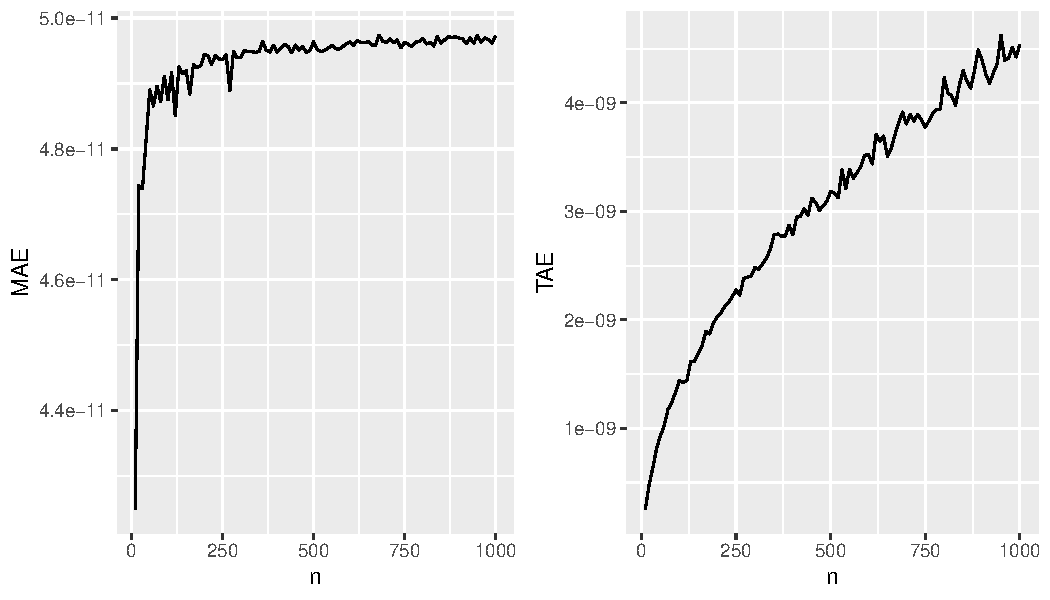
\includegraphics[width=0.95\textwidth]{figures/binom.pdf}
\caption{As $n$ increasing to 1000, the MAE is around $10^{-11}$ and the TAE is around $10^{-9}$.} \label{fig:mae.tae}
\end{center}
\end{figure}


\begin{figure}%[h]
\begin{center}
	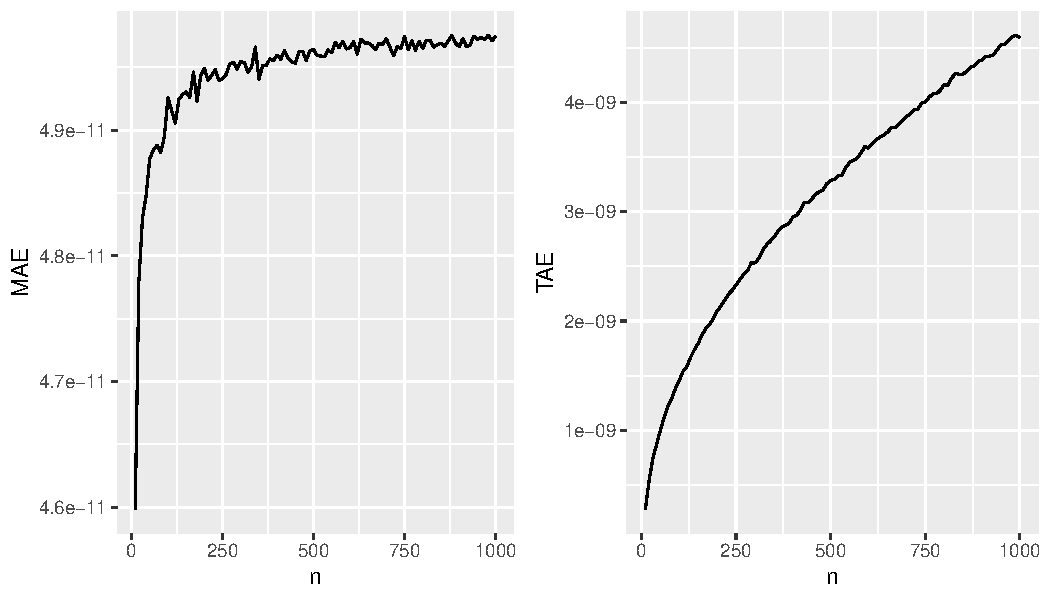
\includegraphics[width=0.95\textwidth]{figures/poib.pdf}
	\caption{Accuracy result of $\dft$ under Poisson binomial scenario.}
	\label{fig:dft.vs.pb}
\end{center}
\end{figure}


\subsection{Accuracy of Normal Approximation and Simulation Method}
%%%%%%%%%%%%%%%%%%%%%%%%%%%%%%%%%%%%%%%%%%%%%%%%%%%%%%%%%%%%%%%%%%%%%%%%%%%%%%%%%%%%%%%%%%%%%%%%%
Among the three computing algorithms we proposed, one of them is able to calculate the exact probability while the other two are approximation methods. Therefore, it is necessary to explore accuracy of the approximation methods under different circumstances. The accuracy metric for $\NA$ is $\MAE$. For $\SIM$ we only consider the maximum probability and probability mass points of 0.95, 0.90 quantiles due to computation capability of device. Probability mass points computed by $\dft$ are considered as true probabilities, denote it as $p_{\textrm{true}}$.
$\MAE$ and $\TAE$ for normal approximation are given by
\begin{equation*}
    \MAE = \max_{\xvec \in \chi}|p_{\NA}(\xvec)-p_{\textrm{true}}(\xvec)|,
\end{equation*}
For simulation method the error metric is given via the difference between the selected probability mass points(maximum, 0.95 and 0.90 quantiles) calculated by $\SIM$ and $\dft$.

For fixed $n$ from 1 to 75 and $m=3$, randomly generate 5000 $\Pmat$'s to exclude the noise effect followed by calculating error metrics with respect to each methods. The results are shown via Figures~\ref{fig:accuracy.sim} and~\ref{fig:mae.na}. In Figure~\ref{fig:accuracy.sim}, we mainly study the relationship between accuracy and simulation times $\mbox{B}$. The top lines in three plots are of $B=10$,  the middle lines are of $B=10^5$ and the rest are of $B=10^7$. Observe that the gap between lines reduces as $n$ increases possibly due to sparsity. The accuracy performance when $B$ is evidently better than when $B$ is small. We can tell from the plots that $B=10^7$ might be a good choice for user since it provide an accuracy error as small as $10^{-5}$.


Specifically, for $\NA$ we introduce a baseline called the Original to express the sparsity of $\PMD$ as $n$ and $m$ increase. The Original is just to estimate all probability mass points by 0's. We can see through the plot the baseline is decreasing which is resulting from sparsity. From Figure~\ref{fig:accuracy.sim}, for given $m$, as $n$ increase the solid line which represent $\NA$ is always under the dashed baseline. The gap between the two lines grows wider as $n$ gets larger for fixed $m$ indicates that $\NA$ is more accurate when $n$ is large regardless of sparsity.

\begin{figure}%[h]
\begin{center}
	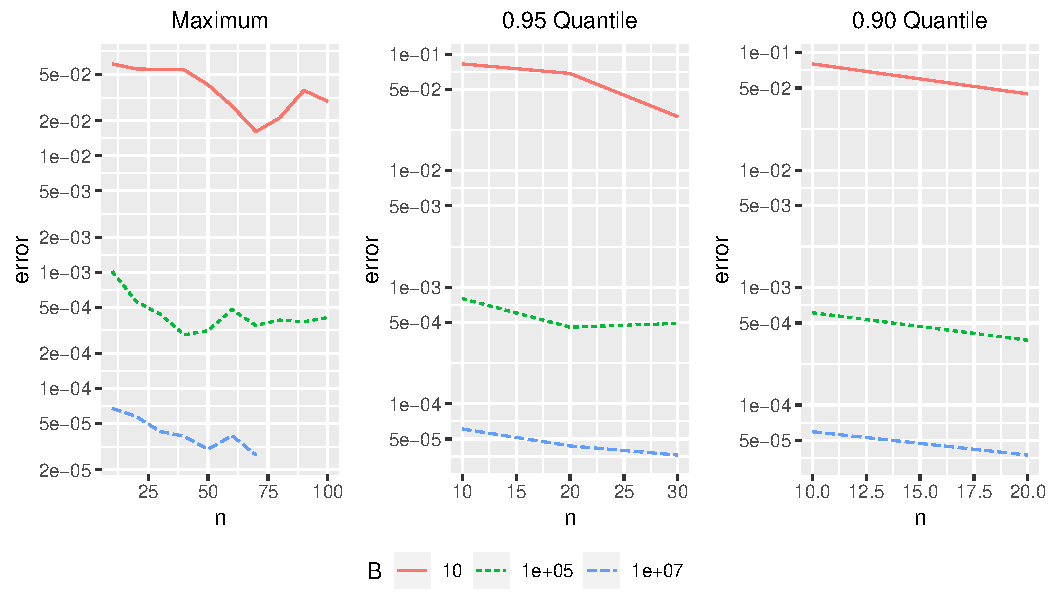
\includegraphics[width=0.95\textwidth]{figures/simulation.pdf}
	\caption{Accuracy of $\SIM$ method based on quantile of $\PMD$ when $m=3$.}
	\label{fig:accuracy.sim}
\end{center}
\end{figure}

\begin{figure}%[h]
\begin{center}
	\includegraphics[width=0.95\textwidth]{figures/mae.pdf}
	\caption{$\MAE$ of $\NA$ compared with baseline (Original).}
	\label{fig:mae.na}
\end{center}
\end{figure}



%%%%%%%%%%%%%%%%%%%%%%%%%%%%%%%%%%%%%%%%%%%%%%%%%%%%%%%%%%%%%%%%%%%%%%%%%%%%%%%%%%%%%%%%%%%%%%%%%
\subsection{Time Efficiency of DFT-CF method}
As a method to compute the whole pmf, we need to consider $\dft$'s time efficiency especially when the dimension is large. The method actually calculates $(n+1)^{m-1}$ probability mass points that includes the possible outcomes of $\PMD$ which is $\binom{n+m-1}{m-1}$. Because it takes every $x_j,j=1,\dots,m-1$ from 0 to $n$. The number $(n+1)^{m-1}$ increases drastically as $m$ gets larger. When $m$ is small, the result is showed by Figure~\ref{fig:time.eff}. When $m$ is moderate ($8 \leq m \leq 20$) or larger, using $\dft$ can be problematic since $(n+1)^{m-1}$ can be enormous such that the device either takes too long to compute nor unable to compute due to exhausted usage of RAM.

We use the same device as for accuracy study to test the time efficiency of $\dft$. Figure~\ref{fig:time.eff} plots the average computing time of 1000 randomly generated $\Pmat$'s using $\dft$. The scale of time is second(s). The following plot (Figure~\ref{fig:time.eff}) shows that the when $m$ is small (less or equal to 4), it is good to use $\dft$ to calculate the entire pmf. As we can see through the plot the computing time for $n=60, m=4$ is 16 seconds which is affordable. Even when $m=5$ and $n=40$ the time is around 100 seconds which is still acceptable. However, when $m=6$ or higher, increasing $n$ can make the computing time huge.


\begin{figure}%[h]
\begin{center}
	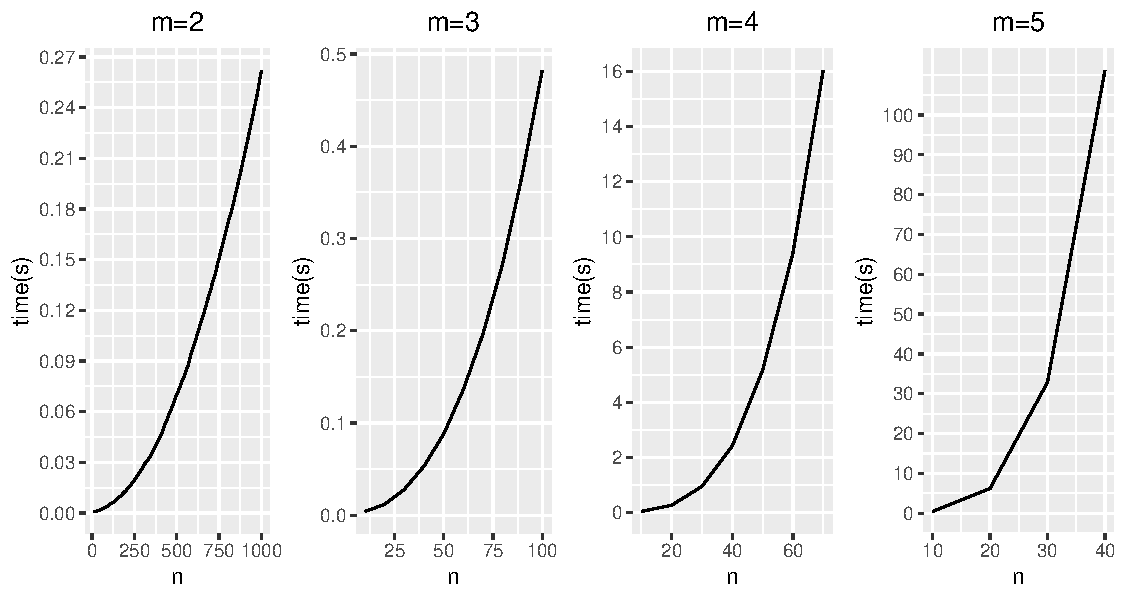
\includegraphics[width=0.95\textwidth]{figures/effi.pdf}
	\caption{Time efficiency study of $\dft$.}
	\label{fig:time.eff}
\end{center}
\end{figure}


%%%%%%%%%%%%%%%%%%%%%%%%%%%%%%%%%%%%%%%%%%%%%%%%%%%%%%%%%%%%%%%%%%%%%%%%%%%%%%%%%%%%%%%%%%%%%%%%%
\subsection{Recommendations}
%%%%%%%%%%%%%%%%%%%%%%%%%%%%%%%%%%%%%%%%%%%%%%%%%%%%%%%%%%%%%%%%%%%%%%%%%%%%%%%%%%%%%%%%%%%%%%%%%
According to the results of accuracy and efficiency study. We hereby give out our recommendations of which method to choose under what circumstances. For small $m$ and moderate $n$, the $\dft$ can be used. Since the computing time is affordable and the method is an exact method that can compute the entire pmf automatically. However when $m$ is moderate or large, this method can be very time consuming and will need a huge RAM. Thus for moderate $m$ ($5 \leq m \leq 20$) and small $n$, we encourage users to use simulation method with $B$ around $10^6$ to calculate partial pmf that is of users' interests. By this way the accuracy will be maintained at a satisfied level and computing time will be affordable. For large $n$ including when $m$ is also large, the $\NA$ is recommended because the accuracy is backed up by central limit theory. If only calculate partial pmf, computing time will not be a concern.

%%%%%%%%%%%%%%%%%%%%%%%%%%%%%%%%%%%%%%%%%%%%%%%%%%%%%%%%%%%%%%%%%%%%%%%%%%%%%%%%%%%%%%
\section{Applications}\label{sec:applications}
%%%%%%%%%%%%%%%%%%%%%%%%%%%%%%%%%%%%%%%%%%%%%%%%%%%%%%%%%%%%%%%%%%%%%%%%%%%%%%%%%%%%%%
\subsection{Calculation of Voting Probability}
In voting scenarios, people always pay attention to the election result. The most thing we usually care about is who will win the election and how many chances each candidate has to win the election. A Poisson Multinomial distribution can fit the situation perfectly under some assumptions.

Suppose a election has $n$ voters and $m$ candidates, there will be $N = \binom{n+m-1}{m-1}$ possible outcomes denoted as $\xvec_r, r = 1, \dots, N$, respectively. Each $\xvec_r$ is a 3 dimension vector that has three elements denoting the number of votes each candidate gets. Assume we know the $\Pmat$ based on prior polls, for example, we can always estimate the approval rate of each candidate in a certain constituency from the monthly polls or exit polls. Then we are able to compute the notional result.

To demonstrate that, suppose we have ten electoral voters and three candidates with $\Pmat$ matrix that has means of column one, two and three to be $0.3631,0.3405$ and $0.2964$, the first five rows are as following,
\begin{equation*}
\begin{pmatrix}
0.071 & 0.589 & 0.340\\
0.365 & 0.195 & 0.440\\
0.445 & 0.505 & 0.050\\
0.353 & 0.382 & 0.265\\
0.620 & 0.111 & 0.269
    \end{pmatrix}
\end{equation*}
To compute the probability of each candidate winning the election, just need to introduce constraints. For instance, under the constraint $\chi_1 = \left\{\text{the first element is the largest one}\right\} = \left\{x_1>x_2, x_1>x_3; x_1, x_2,x_3 \in \left\{0,\dots,10\right\}\right\}$, we are able to compute the winning rate of the first candidate is
\begin{equation*}
\Pr(\text{the 1st candidate wins}) = \sum_{\xvec \in \chi_{1}} p(\xvec) = 0.3429
\end{equation*}
Similarly, the probabilities for the second candidate and the third candidate to win are $0.2745$ and $0.2001$. Additionally, the most possible result is $\xvec = (4,3,3)$, which has probability 0.08546.




%%%%%%%%%%%%%%%%%%%%%%%%%%%%%%%%%%%%%%%%%%%%%%%%%%%%%%%%%%%%%%%%%%%%%%%%%%%%%%%%%%%%%%
\subsection{Statistical Inference for Aggregated Data}\label{sec:model.est.inf}	
First introduce the ``Logistic-like" model to fit a given aggregated dataset with selected features and a categorical response variable that has $m$ categories.
By dividing the rows of our data into $H$ groups $G_1,\dots,G_{S}$ via some given criterion, the group size of each group is $s_i,i=1,\dots,S$. Each $s_i$ are positive integer but not necessarily equal to each other. Let the quantity for each category of group $G_i$ be $\xvec^{(i)} = (x_1^{(i)}, \dots, x_m^{(i)})'$, $m$ is the category number. Denote $\Hmat^{(i)}$ to be the covariate matrix of $G_i$, then $\Hmat^{(i)} = (\onevec, \hvec_{1}^{(i)},\dots,\hvec_{s_i}^{(i)})'$ is a $s_i \times v$ matrix with first column being $\onevec$, where $v$ equals to the number of covariates plus one. Let $\Pmat^{(i)} = (p_{jk}^{(i)})$ be the SPM for group $G_i$, $i = 1, \dots, S$, $j = 1,\dots ,s_i$ and $k = 1,\dots, m$. Let the probability of getting $\xvec^{(i)}$ for group $G_i$ be $p(\xvec^{(i)})$. The total log-likelihood for all groups can be computed as
\begin{equation*}
\loglik = \sum_{i=1}^{S}\loglik_i = \sum_{i=1}^{S}\log p(\xvec^{(i)})
\end{equation*}
Where $p(\xvec^{(i)})$ can be computed via Poisson Multinomial distribution with SPM $\Pmat^{(i)}$. Set category $m$ as baseline and use softmax function to form the $\Pmat^{(i)}$ for each group through parameter $\betavec = (\betavec_1, \dots, \betavec_{m-1})$ as
\begin{align*}
    p_{j k}^{(i)} = \frac{\exp{\left(\hvec_{j}^{(i)} \betavec_{k}\right)}}{1 + \sum_{k=1}^{m-1}\exp{\left( \hvec_{j}^{(i)} \betavec_{k} \right)}}
    \quad k \neq m \quad \text{and } \quad
    p_{i,m}^{(i)} = \frac{1}{1 + \sum_{k=1}^{m-1}\exp{\left( \hvec_{j}^{(i)} \betavec_{k} \right)}}
\end{align*}

Then we are able to estimate our parameters on the direction of minimizing total log-likelihood and finally get our estimate $\wh{\Pmat}^{(i)}$.

In the rest of this part, we apply the model to the dataset ``ai4i" \cite{Dua:2019}. The dataset ``ai4i" is a synthetic machine failure dataset that reflects real predictive maintenance data encountered in industry. The data consists of 10000 products(rows) and 14 features(columns) including Product type, Air temperature, Process temperature, Rotational speed and others.

For demonstration purpose, here we only use the first 1000 rows and Product type as response variable, Air temperature and Process temperature as covariates. The feature Product type is categorical and has three levels, ``M", ``L", ``H", we denote them as category 1, 2, 3 for simplicity. The number of products that fall in category 1, 2, and 3 are 285, 601, and 114. The other two features are continuous.


We randomly divide the dataset into 100 groups $G_1,\dots,G_{100}$, the smallest group has size of three rows and the largest one has 18 rows. Note that readers can use other criterion to divide the dataset by their own. Notice the covariate number is three including intercept and the response has three categories, thus the dimension of our parameter matrix $\betavec$ will be $3 \times 2$ if we set category 3 as baseline.

The estimates of the parameters are
\begin{equation*}
\wh{\betavec} =
\begin{pmatrix}
 1.07484986 & 2.2820922 \\
 1.62342045 & 1.9108976 \\
 -0.06277732 &-0.8455964\\
\end{pmatrix}
\end{equation*}
The corresponding $\wh{\Pmat}^{(1)}$ and $\wh{\Pmat}^{(5)}$ for group 1 and group 5 are
\begin{equation*}
    \wh{\Pmat}^{(1)} = \begin{pmatrix}

 0.11914 & 0.63310 & 0.24776\\
 0.12326 & 0.57268 & 0.30406\\
 0.14809 & 0.47560 & 0.37631\\
 0.14504 & 0.56971 & 0.28525\\
 0.12451 & 0.54095 & 0.33454\\
 0.04170 & 0.55944 & 0.39886\\
 0.03559 & 0.53568 & 0.42873\\
 0.04890 & 0.54668 & 0.40442
    \end{pmatrix}, \quad
    \wh{\Pmat}^{(5)} = \begin{pmatrix}
 0.15604 & 0.70766 & 0.13630\\
 0.14469 & 0.73976 & 0.11555\\
 0.11246 & 0.67372 & 0.21382\\
 0.12036 & 0.64885 & 0.23079\\
 0.11263 & 0.61304 & 0.27433\\
 0.11563 & 0.55029 & 0.33408\\
 0.11774 & 0.61672 & 0.26554\\
 0.15071 & 0.52510 & 0.32419\\
 0.13878 & 0.56645 & 0.29477\\
 0.08194 & 0.54561 & 0.37245\\
 0.06307 & 0.58191 & 0.35502
    \end{pmatrix}
\end{equation*}
For group 1 and 5, $\xvec^{(1)} = (1,5,2)'$ and $\xvec^{(5)} = (2,6,3)'$, so $p(\xvec^{(1)}) = 0.070$, $p(\xvec^{(5)}) = 0.067$.
%%%%%%%%%%%%%%%%%%%%%%%%%%%%%%%%%%%%%%%%%%%%%%%%%%%%%%%%%%%%%%%%%%%%%%%%%%%%%%%%%%%%%%

%%%%%%%%%%%%%%%%%%%%%%%%%%%%%%%%%%%%%%%%%%%%%%%%%%%%%%%%%%%%%%%%%%%%%%%%%%%%%%%%%%%%%%
\subsection{Uncertainty Quantification in Classification}
In machine learning classification problem with multiple labels, for each unit in the test set, the probability of the unit belongs to each class is computed. Usually, the predicted class is assigned as the highest probability. Using the soft classifiers, the unit class is randomly assigned according to the predicted probabilities, leading to randomness in the confusion matrix. The PMD can be used to characterize the distribution of the counts in the confusion matrix.

In this section, we consider an Electroluminescence (EL) image classification example to illustrate the usage of PMD in machine learning classification problems. In the photovoltaic (PV) reliability study, the EL image is an important data type that reveal information about the PV health status. Because disconnected parts do not irradiate, the darker areas in EL images indicate defective cells. The EL imaging provide visual inspection of solar panels and is a non-destructive technology for failure analysis of PV modules \shortcite{Deitsch2019}.

The work of \shortciteN{Deitsch2019}, \shortciteN{Buerhop2018}, and \shortciteN{Deitsch2021} provide a public dataset of solar cells extracted from high resolution EI images of PV modules (\url{https://github.com/zae-bayern/elpv-dataset}). In total there are 2624 images. All images are preprocessed with respect to size and are eliminated distortion induced by the camera lens used to capture the EL images. Each image is manually labeled  with its degree of defectiveness. The degree of defectiveness is determined by two questions. The first is how do evaluators think the status of the solar cells, functional or defective; the second is how they are confident about their assessments. In total there are four labels as shown in Table \ref{tbl:el.label} and we marked them as Class A-D.

\begin{table}%[h!]
\caption{Partitioning of solar cells into functional and defective, with an additional self-assessment on the rater's confidence after visual inspection. Non-confident decisions obtain a weight lower than 100\% for the evaluation of the classifier performance.}\label{tbl:el.label}
\begin{center}	
\begin{tabular}{c|c|c|c|c}
		\hline
		\hline
		Condition  & Confident?  &  Label $p$ & Weight $w$ & Class \\
		\hline
		\multirow{2}{*}{functional} & Yes & functional & 0\% & A\\
		& No& defective  & 33\% & B\\
		\hline
		\multirow{2}{*}{defective} & No & defective & 67\% & C\\
		& Yes & defective & 100\%  &D\\
		\hline
		\hline
	\end{tabular}
\end{center}
\end{table}
%According to the probability how likely the product is defective, we assign four labels to sollar cells, 0\%, 33.33\%, 66.66\%, 100\%.

We split our data to training data (80\%) and test data (20\%), then train a CNN model on the training set. In CNN model, we use Relu activation function and set the kernel size $3 \times 3$ and stride $1 \times 1$. For each image in the testing set, the model provides a probability that the prediction belongs to each class. Table~\ref{tbl:elpmat} provides a subset of the CNN model output. For true class for the first sample in Table~\ref{tbl:elpmat} is A. If we predict the class of the first sample using the highest probability, then the prediction is A and there's no randomness. If we allow the model to make predictions based on the probability vector as shown in the first row then there are randomness in the confusion matrix. We can consider the confusion matrix to follow a PMD distribution then we can quantify the uncertainty in confusion matrix using PMD.

Figure~\ref{fig:confusion.hist} shows the marginal probability of each cell. For example, in the first row first column panel cell in Figure~\ref{fig:confusion.hist}, we know the possible counts that the model correctly predict class A as well as the corresponding probability. In this way, we have a uncertainty quantification in the confusion matrix.


\begin{table}%[ht]
\begin{center}
\caption{An example of the probability vectors of a subset in testing set from the trained CNN model.}\label{tbl:elpmat}
\begin{tabular}{rrrrr}
  \hline\hline
 & A & B & C & D \\
  \hline
1 & 0.9230 & 0.0366 & 0.0107 & 0.0297 \\
  2 & 0.0736 & 0.0802 & 0.0513 & 0.7950 \\
  3 & 0.0000 & 0.0016 & 0.0006 & 0.9978 \\
  4 & 0.9170 & 0.0537 & 0.0062 & 0.0231 \\
  5 & 0.9579 & 0.0239 & 0.0070 & 0.0112 \\
  6 & 0.8991 & 0.0347 & 0.0132 & 0.0530 \\
   \hline\hline
\end{tabular}
\end{center}
\end{table}


\begin{figure}
\begin{center}
	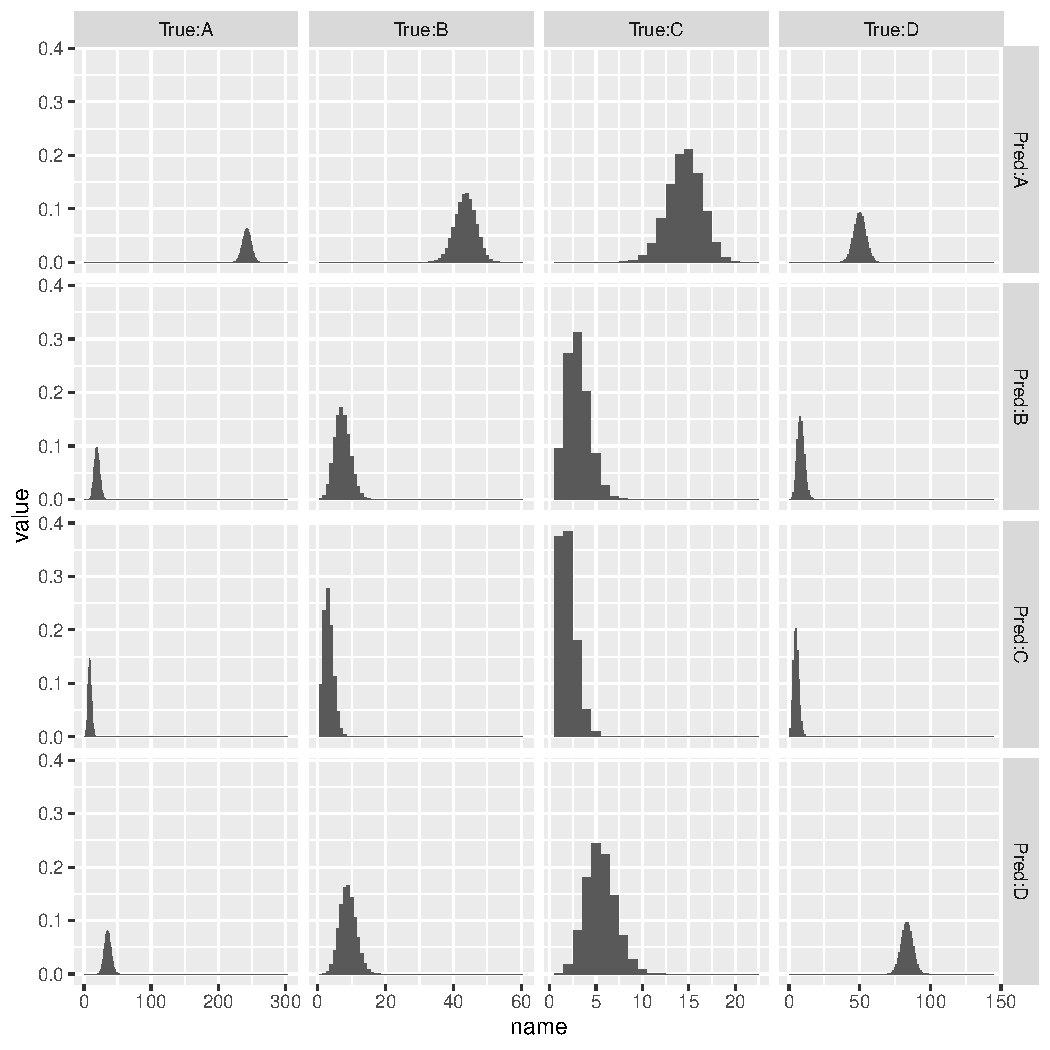
\includegraphics[width=0.9\textwidth]{figures/Confusionbar.pdf}
	\caption{The barplot shows the confusion matrix prediction. For each panel cell, the plot shows the corresponding prediction counts fall in this cell as well as their probability. We also present the mean and 95\% naive prediction interval.}
	\label{fig:confusion.hist}
\end{center}
\end{figure}


%%%%%%%%%%%%%%%%%%%%%%%%%%%%%%%%%%%%
\section{Illustrations of the R Package}\label{sec:rpackage}
%%%%%%%%%%%%%%%%%%%%%%%%%%%%%%%%%%%%%%%%%%%%%%%%%%%%%%%%%%%%%%%%%%%%%%%%%%%%%%%%%%%%%%%%%%%%%%%%%
We develop an R package $\textrm{PoissonMultinomial}$ specifically computes probability density function for $\PMD$ with corresponding $\Pmat$ using the methods described by this paper. The fast Fourier transformation algorithm are implemented in C.

There are three major functions in the package. $\code{dpmd}$ is a function to compute pmf, $\code{ppmd}$ is for cdf and one can use $\code{rpmd}$ to generate $\PMD$ random samples. User has to specify $\Pmat$ so that a $\PMD$ can be determined. With unspecified $\xvec$, $\code{dpmd}( )$ will automatically calculate the whole pmf and the output will be a multi-dimensional array. If user inputs $\xvec$, the output of $\code{dpmd}( )$ will be partial pmf chosen by $\xvec$. User can also select all methods we list in this paper to compute the pmf or cdf. Notice only $\dft$ can automatically compute the whole pmf and it is the most efficient way for this job as well. The function $\code{ppmd}$ uses same method as $\code{dpmd}$ to compute the probability $\Pr(\Xvec \leq \xvec)$ and the function $\code{rpmd}$ generates random samples from $\PMD$.  Examples of using $\code{dpmd}$ is following,

First, $\code{pp}$ is an input matrix that specifies a $\PMD$. It looks as
\begin{verbatim}
  pp=matrix(c(0.1, 0.1, 0.1, 0.7,
              0.1, 0.3, 0.3, 0.3,
              0.5, 0.2, 0.1, 0.2),
              byrow=T, ncol=4, nrow=3)
\end{verbatim}
%$$
%\begin{pmatrix}
%0.1 & 0.1 & 0.1& 0.7\\
%0.1 &0.3 & 0.3 & 0.3\\
%0.5  &0.2 & 0.1 & 0.2
%\end{pmatrix}
%$$
and $\xvec=(0,0,1,2)'$. Then the codes of using $\code{dpmd}$ to calculate pmf, is given as following
\begin{verbatim}
  dpmd(pmat = pp)
  dpmd(pmat = pp, xmat = x)
  dpmd(pmat = pp, xmat = x, method = "NA" )
  dpmd(pmat = pp, method = "SIM", B = 1e3)
  dpmd(pmat = pp, xmat = x, method = "SIM", B = 1e3)
\end{verbatim}
The first line computes the whole pmf, the second one computes partial pmf of given $\xvec$, the rest of the codes just do the similar job using $\NA$ and $\SIM$.
We shall demonstrate the one to one map between the output and the pmf of an $n \times m$ $\PMD$. First we have a location indicator vector $v = (v_1, \dots, v_{m-1})'$ and an $\xvec=(x_1,\dots,x_m)'$, let $v_j-1 = x_j, j =1,\dots,m-1$ then the array element with location $v$ has the value of $\Pr(X=\xvec)$. We further illustrate this map via the $\Pmat$ given above.

The $\Pmat$ is $3 \times 4$ so the output of $\code{dpmd}$ is a $4 \times 4 \times 4$ dimensional array listed in figure (a), (b), (c), (d). Since the input $\code{pp}$ is dimension $3 \times 4$, the output is an $4 \times 4 \times 4$ array. First consider the element of row 3 column 2 in (a). Then the first two elements of $v$ is 3 and 2. the third element depends on the comma number on the top of each figure. On the top of (a) there are two commas followed by 1, thus the third element of $v$ is 1. Now we have constructed $v = (3,2,1)$, then we minus 1 on each element we get $(2,1,0)=\xvec'$ which is the corresponding probability mass point. So far we can get the element that has location indicated by $v=(3,2,1)$ is 0.022 and we have $\Pr(X=(2,1,0)')=0.022$. In the other direction, if we want to know the probability of $X=\xvec=(0,3,0)'$ we need to construct its corresponding $v$, which can be computed by plus 1 to each element in $\xvec$ so that we get $v=(1,4,1)$. The $v$ we just constructed indicates a location of (1,4,1) of our array. That location is the first row, 4th column in the $\text{, , 1}$ figure which has value 0.006.

\begin{verbatim}
  res=dpmd(pmat=pp)
  res
  , , 1                              , , 2
        [,1]  [,2]  [,3]  [,4]             [,1]  [,2]  [,3] [,4] 
  [1,] 0.042 0.090 0.054 0.006       [1,] 0.069 0.084 0.015    0 
  [2,] 0.125 0.148 0.023 0.000       [2,] 0.138 0.042 0.000    0 
  [3,] 0.052 0.022 0.000 0.000       [3,] 0.021 0.000 0.000    0 
  [4,] 0.005 0.000 0.000 0.000       [4,] 0.000 0.000 0.000    0 
  , , 3                              , , 4                     
        [,1]  [,2] [,3] [,4]               [,1] [,2] [,3] [,4]
  [1,] 0.030 0.012    0    0         [1,] 0.003    0    0    0 
  [2,] 0.019 0.000    0    0         [2,] 0.000    0    0    0 
  [3,] 0.000 0.000    0    0         [3,] 0.000    0    0    0 
  [4,] 0.000 0.000    0    0         [4,] 0.000    0    0    0 
\end{verbatim}


%\begin{figure}
%  \begin{subfigure}{8cm}
%    \centering
%    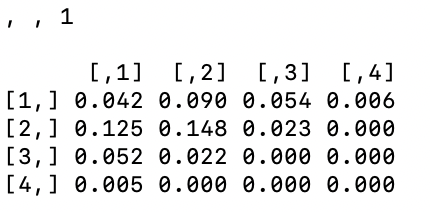
\includegraphics[width=7cm]{figures/1.png}
%    \caption{ }
%  \end{subfigure}
%  \begin{subfigure}{9cm}
%    \centering
%    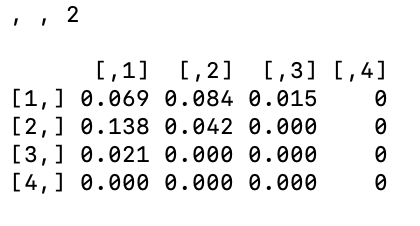
\includegraphics[width=7cm]{figures/2.png}
%    \caption{ }
%  \end{subfigure}
%  \begin{subfigure}{8cm}
%    \centering
%    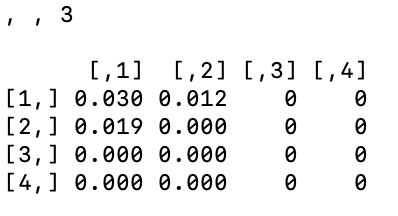
\includegraphics[width=7cm]{figures/3.png}
%    \caption{ }
%  \end{subfigure}
%  \begin{subfigure}{9cm}
%    \centering
%    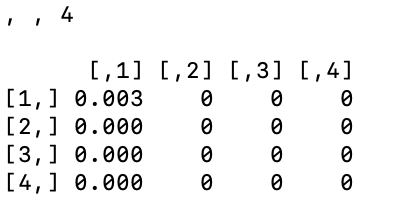
\includegraphics[width=7cm]{figures/4.png}
%    \caption{ }
%  \end{subfigure}
%\end{figure}



%%%%%%%%%%%%%%%%%%%%%%%%%%%%%%%%%%%%%%%%%%%%%%%%%%%%%%%%%%%%%%%%%%%%%%%%%%%%%%%%%%%%%%%%%%%%%%%%%
\section{Conclusions and Areas for Future Research}\label{sec:conclusion}
%%%%%%%%%%%%%%%%%%%%%%%%%%%%%%%%%%%%%%%%%%%%%%%%%%%%%%%%%%%%%%%%%%%%%%%%%%%%%%%%%%%%%%%%%%%%%%%%%

We develop three methods that can be useful for computing the pmf of the PMD, which is challenging to compute but useful in many application scenarios. We include the three methods we designed in an R package. Among the methods, $\dft$ is an exact method, $\SIM$ is a simulation method and $\NA$ is a method using approximation theories. The accuracy and efficiency of the methods are guaranteed under given circumstances. We recommend users to use $\dft$ when $m$ is small, use $\SIM$ when $m$ is moderate and $n$ is small, use $\NA$ when $n$ is large. However, there are still some fields remain to be explored. The computing speed of $\dft$ can be improved using more efficient Fourier transformation algorithms or we could find a way to calculate only the $\binom{n+m-1}{m-1}$ possible outcomes rather than $(n+1)^{m-1}$ probability mass points which contains a large amount of points have values equal to 0. $\SIM$ method is still time consuming although it can compute some cases that $\dft$ are unable to, once we develop more efficient exact algorithms, $\SIM$ could be replaced. Untill now, we are still unable to compute the pmf of $\PMD$ when $m$ is large due to the computational limit of machines, this area remains to be disclosed.

%%%%%%%%%%%%%%%%%%%%%%%%%%%%%%%%%%%%%%%%%%%%%%%%%%%%%%%%%%%%%%%%%%%%%%%%%%%%%%%%%%%%%%%%%%%%%%%%%%%%%%%%%%%%%%%%%%%%

%\section*{Acknowledgments}
%%%%%%%%%%%%%%%%%%%%%%%%%%%%%%%%%%%%%%%%%%%%%%%%%%%%%%%%%%%%%%%%%%%%%%%%%%%%%%%%%%%%%%%%%%%%%%%%%%%%%%%%%%%%%%%%%

%\bibliographystyle{apacite}


\bibliographystyle{chicago}
%\bibliography{refs.BIB}	
\bibliography{refs}	

\end{document}

%%%%%%%%%%%%%%%%%%%%%%%%%%%%%%%%%%%%%%%%%%%%%%%%%%%%%%%%%%%%%%%%%%%%%%%%%%%%%%%%%%%%%%%%%%%%%%%%%%%%%%%%%%%%%%%%%%%%%%%%%%%%%%%%%%%%%%%

